
%(BEGIN_QUESTION)
% Copyright 2014, Tony R. Kuphaldt, released under the Creative Commons Attribution License (v 1.0)
% This means you may do almost anything with this work of mine, so long as you give me proper credit

Suppose that an electric heater, which is nothing more than a large resistor, dissipates 500 watts of power when directly connected to a 110 volt source:

$$\includegraphics[width=15.5cm]{i01139x01.eps}$$

Now suppose that exact same heater is connected to one end of a long two-wire cable, which is then connected to the same 110 volt source.  Assuming that each conductor within the cable has an end-to-end resistance of 3 ohms, how much power will the heater dissipate?

$$\includegraphics[width=15.5cm]{i01139x02.eps}$$

\underbar{file i01139}
%(END_QUESTION)





%(BEGIN_ANSWER)

$P$ = 321.1 watts

%(END_ANSWER)





%(BEGIN_NOTES)

The purpose of this question, besides providing a good problem-solving exercise for students, is to get them to realize one of the practical implications of power-line resistance.

%INDEX% Electronics review: series and parallel circuits

%(END_NOTES)


